%% Modified LaTeX-Beamer template, stolen from the SDQ group and
%% adapted by Philipp Becker 
%% Original Statement:

%%------------------------------------------------------------
%% LaTeX-Beamer template for KIT design
%% by Erik Burger, Christian Hammer
%% title picture by Klaus Krogmann
%%
%% version 2.5
%%
%% mostly compatible to KIT corporate design v2.0
%% http://intranet.kit.edu/gestaltungsrichtlinien.php
%%
%% Problems, bugs and comments to
%% burger@kit.edu
%%------------------------------------------------------------
%% Class options
%%   aspect ratio options: 
%%   -- 16:9 (default)
%%   -- 4:3
%%   language options: 
%%   -- en (default)
%%   -- de
%%   position of navigation bar:
%%   -- navbarinline (default): bottom of the white canvas
%%   -- navbarinfooter : more compressed variant inside the footer
%%   -- navbarside : side bar at the left of the white canvas
%%   -- navbaroff : none
%% example: \documentclass[16:9,de,navbarinfooter]{sdqbeamer}

\documentclass[navbarinfooter, 12pt]{sdqbeamer}
 
%% TITLE PICTURE

% if a custom picture is to be used on the title page, copy it into the 'logos'
% directory, in the line below, replace 'myimage' with the 
% filename (without extension) and uncomment the following line
% (picture proportions: 63 : 20 for standard, 169 : 40 for wide
% *.eps format if you use latex+dvips+ps2pdf, 
% *.jpg/*.png/*.pdf if you use pdflatex)

%\titleimage{alr_logo}

%% GROUP LOGO 

% for a custom group logo, copy your file into the 'logos'
% directory, insert the filename in the line below and uncomment it

% \grouplogo{mylogo}

% (*.eps format if you use latex+dvips+ps2pdf,
% *.jpg/*.png/*.pdf if you use pdflatex)

%% GROUP NAME

% for groups other than SDQ, please insert in the line below and uncomment it
% \groupname{}

% the presentation starts here 

\title[Short Title]{Recursive Surrogate-Modeling for Stochastic Search}
\subtitle{Intermediate Presentation - Bachelor Thesis}
\author{Philipp Theyssen}

% Bibliography 

\usepackage[citestyle=authoryear,bibstyle=numeric,hyperref,backend=biber]{biblatex}
\usepackage{xcolor}
\usepackage{tikz}
\usepackage{caption}
% \usepackage{pgfpages}
% \setbeameroption{show notes on second screen=right}
\addbibresource{presentation.bib}
\bibhang1em


\begin{document}

%title page
\KITtitleframe
% table of contents
\section{Outline}
\begin{frame}{Outline}
 \begin{itemize}
  \item Motivation
  \item Introduction
  \item Recursive Surrogate-Modeling for MORE
  \item Preliminary Results
  \item Outlook
  \end{itemize}
  % \note{test note}
\end{frame}


%%%%%%%%%%%%%%%%%%%%%%%%%%%%%%%%%%%%%%%%%%%%%%%%%%%%%%%%%%%%%%%%%%%%%%%%%%%%%%%%
%%%%%%%%%%%%%%%%%%%%%%%%%%%%%%%%%%%%%%%%%%%%%%%%%%%%%%%%%%%%%%%%%%%%%%%%%%%%%%%%
% General todo:
% TODO: use ispell to check every word
% TODO: add reference for pictures I used
% TODO: add figure for correlated surrogate models (contour lines)
%%%%%%%%%%%%%%%%%%%%%%%%%%%%%%%%%%%%%%%%%%%%%%%%%%%%%%%%%%%%%%%%%%%%%%%%%%%%%%%%
%%%%%%%%%%%%%%%%%%%%%%%%%%%%%%%%%%%%%%%%%%%%%%%%%%%%%%%%%%%%%%%%%%%%%%%%%%%%%%%%

\section{Motivation}

\begin{frame}{Autonomous Robots: Key Challenges}
\begin{columns}[c]
  \begin{column}{7cm}
    Main tasks for autonomous robots: \\
      \begin{itemize}
      \item Modeling
      \item Predicting
      \item Decision making
      \end{itemize}
  \end{column}
  \begin{column}{5cm}
    \begin{figure}[ht]
      \centering
      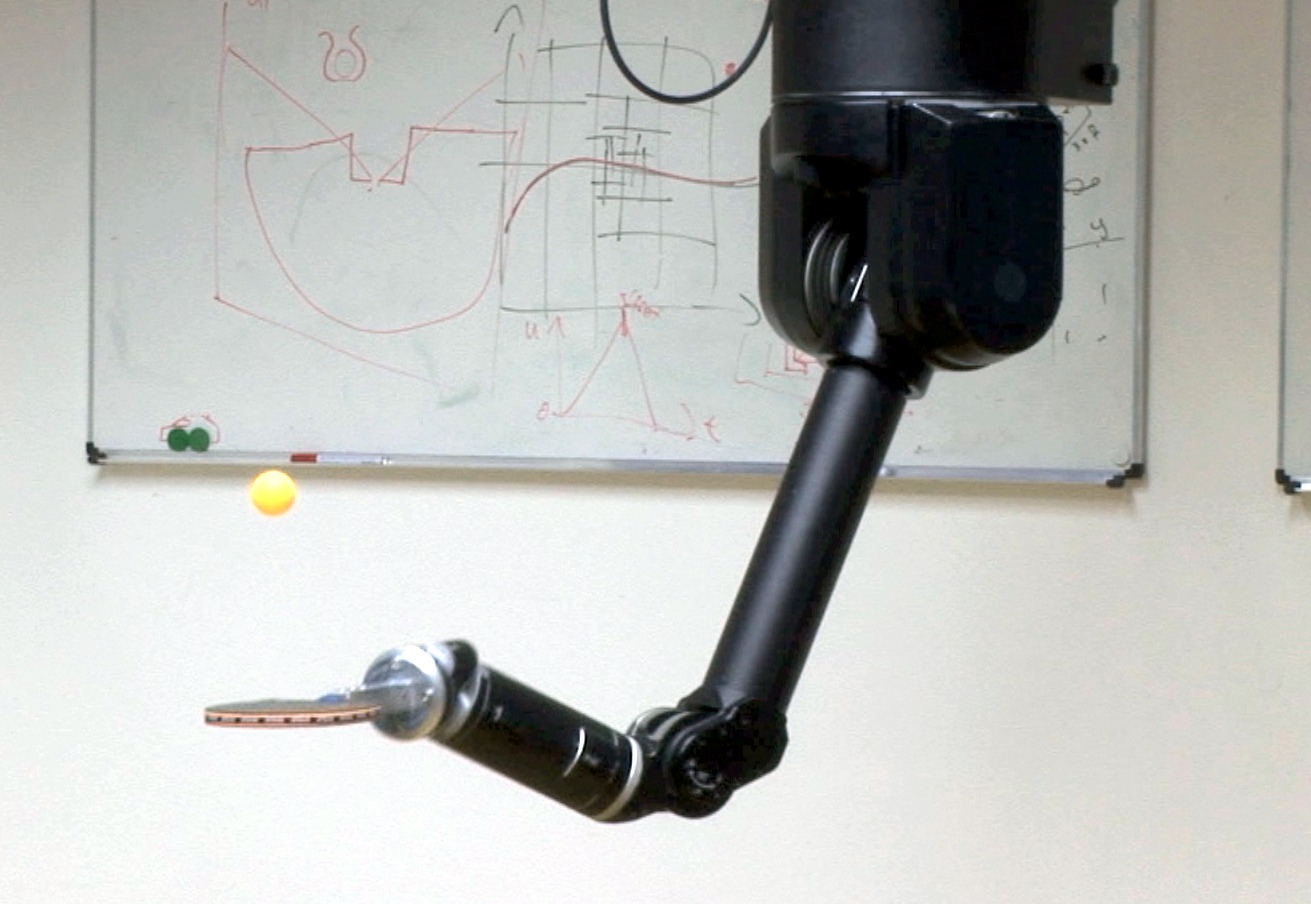
\includegraphics[height=3.5cm]{figures/robot_table_tennis.png}
    \end{figure}

  \end{column}
\end{columns}  
\begin{block}{Challenges}
  \begin{itemize}
  \item fully autonomous (no human in the loop)
  \item uncertainty, sensor noise
  \item data efficiency
  \end{itemize}
\end{block}
\end{frame}


\begin{frame}{Sample Efficiency Problem}
\begin{itemize}
\item \textbf{sample efficiency} for robot learning
\item real-world samples are expensive in time, labor and finances
\item robot hardware is expensive, needs careful maintenance
\item working with non-industrial robots
\end{itemize}
\end{frame}


%\begin{frame}{Policy Search with Stochastic optimizer}
%  \alert{TODO:talk about interaction with environment, change this slide because this is more model based PS } \\
%  \begin{itemize}
%  \item learn parametrized policy $\pi(x_t, \theta)$ to create samples in parameter space
%  \end{itemize}
%  \centering
%  \begin{tikzpicture}
%    \draw (0,0) node {$ p(x_{t+1} | x_t, u_t) \quad \quad u_t \; = \; \pi(x_t, \theta) $};
%    \draw [->][very thick] (-2.9,-1) -- (-3.4,-0.3);
%    \draw [->][very thick] (-2.36,-1.05) -- (-1.7,-0.3);    
%    \draw (-2.7,-1.3) node {Probabilistic transition function};
%    \draw (2,0) node {Control}
%    \draw 
%    % $$ x_{t+1} = f(x_t, u_t) + w,  u_t = \pi(x_t, \theta) $$
%  \end{tikzpicture}
%  \begin{block}{Policy Search}
%    Find policy parameters $\theta^*$ that maximizes expected accumulated reward
%  \end{block}  
%\end{frame}

\section{Introduction}

\begin{frame}{Stochastic search}
  \begin{block}{Stochastic search}
    \begin{itemize}
    \item optimize objective function $f(\mathbf{x}): \mathbb{R}^n \rightarrow \mathbb{R}$
    \item learn policy $\pi(\mathbf{x})$ (search distribution) over parameter space of objective function
    \item black-box optimizer: only evaluate objective function (no gradients)
    \item iteratively update search distribution (policy)
    \end{itemize}
  \end{block}
\textbf{Examples} \\
    \begin{itemize}
    \item learn motor skills with Dynamic Movement Primitives
    \end{itemize}
\end{frame}

\begin{frame}{MORE Algorithm for Policy Search}
\begin{block}{MORE-Framework for Constraint Optimization Problem}
  \begin{align*}
    \max_{\pi} \int \pi(\mathbf{x}) f(\mathbf{x}) dx \quad \quad  &\rightarrow \text{Maximize objective} \\
    \text{ s.t. KL}(\pi(\mathbf{x})||\pi_{t-1}(\mathbf{x})) \leq \epsilon \quad \quad &\rightarrow \text{bound between old and new policy} \\
    H(\pi) \geq \beta \quad \quad  &\rightarrow \text{lower entropy bound} \\ 
    1 = \int \pi(\mathbf{x}) dx  \quad \quad  &\rightarrow \text{distribution requirement}
  \end{align*}
\end{block}

$\rightarrow$ cannot evaluate integral in optimization problem \\
$\rightarrow$  approximate objective with quadratic surrogate model
\end{frame}


\begin{frame}{Solve Dual Function}
\begin{block}{Surrogate Model}
  $$f(\mathbf{x}) \approx \hat{f}(\mathbf{x}) = \mathbf{x}^T \mathbf{A} \mathbf{x} + \mathbf{x}^T \mathbf{a} + a $$
\end{block}
  \textbf{New policy:}
    $$ \pi_{t+1} = \mathcal{N}(\mu_{t+1}, \Sigma_{t+1}) $$
    $$ \mu_{t+1} = B_t^{-1} b_t   \quad \quad  \Sigma_{t+1} = B_t^{-1} $$
    \text{with}
    $$ B_t = (\eta \Sigma_t^{-1} + \textbf{A}) / (\eta + \omega) $$
    $$ b_t = (\eta \Sigma_t^{-1} \mu_t + \textbf{a}) / (\eta + \omega) $$
    and $\eta, \omega$ Lagrangian multipliers
\end{frame}

\begin{frame}{MORE Algorithm}
  \begin{block}{Iteration Step}
    \begin{enumerate}
    \item Draw samples from search distribution + evaluate objective function
    \item Estimate surrogate model using samples + values
    \item Use surrogate model to solve optimization problem analytically
    \item update search distribution
    \end{enumerate}
  \end{block}
\end{frame}


\begin{frame}{Surrogate Model}
\begin{columns}[c]
  \begin{column}{8cm}
    \begin{itemize}
    \item local approximation of objective function
    \item $\mathcal{O}(n^2)$ parameters to estimate
    \item KL-bound avoids over-exploitation of surrogate model 
    \end{itemize}
  \end{column}
  \begin{column}{5cm}
    
\includegraphics[height=5cm]{figures/Surrogate_Model.png}
  \end{column}
\end{columns}  
\end{frame}


\begin{frame}{Surrogate Model}
  \begin{itemize}
  \item current approach: learn new model in each iteration
  \item subsequent models are locally correlated
  \end{itemize}
%  \alert{ TODO: add figure of multiple surrogate models to stress correlation}
  \begin{alertblock}{Central Question}
    Can we improve sample efficiency by recursively estimating \\
    the surrogate model?
  \end{alertblock}  
\end{frame}


%%%%%%%%%%%%%%%%%%%%%%%%%%%%%%%%%%%%%%%%%%%%%%%%%%%%%%%%%%%%%%%%%%%%%%%%%%%%%%%%
%%%%%%%%%%%%%%%%%%%%%%%%%%%%%%%%%%%%%%%%%%%%%%%%%%%%%%%%%%%%%%%%%%%%%%%%%%%%%%%%


\section{Recursive Surrogate-Modeling for MORE}

\begin{frame}{Linear regression model}
  \begin{block}{Regression problem}
    \begin{align*}
      y_k &=  \mathbf{x}^T \mathbf{A} \mathbf{x} + \mathbf{x}^T \mathbf{a} + a + \epsilon_k \\
      \theta &= (\mathbf{A}, \mathbf{a}, a)
   \end{align*}
   $\rightarrow$ estimate parameters $\theta$ from samples + objective values \\
   $\rightarrow$ measurement noise $\epsilon_k$ is zero mean
   Gaussian $\epsilon_k \sim N(0, \sigma^2)$
  \end{block}
  % $\rightarrow$ we estimate $ 1 + d + d(d + 1) / 2$ parameters, $\mathbf{x} \in \mathbb{R}^d$
\end{frame}

\begin{frame}{Linear regression}
  \begin{block}{Bayesian Estimation}
    \begin{align*}
      p(\mathbf{\theta}) &= \text{N}(\mathbf{\theta} | \textbf{m}_0, \textbf{P}_0)
      \; \; \; \quad \rightarrow \text{prior} \\      
      p(y_k | \mathbf{\theta}) &= \text{N}(y_k | \textbf{H}_k \mathbf{\theta}, \sigma^2)
                                 \quad \rightarrow  \text{likelihood} \\ 
      p(\theta | y_{1:T}) &= \text{N}(\theta | y_{1:T}) \quad \quad \quad \rightarrow \text{posterior}
  \end{align*}
  $\textbf{H}_k$ matrix with samples (design matrix)
\end{block}
\end{frame}


\begin{frame}{Least Squares}
  \begin{block}{Least Squares solution}
    \textit{batch solution} with application of Bayes' rule
    \begin{align*}
      p(\theta | y_{1:T}) &\propto p(\theta) \prod^T_{k=1} p(y_k|\theta)  \\
                          &= \text{N}(\theta | \textbf{m}_0, \textbf{P}_0)
                            \prod^T_{k=1} \text{N}(y_k | \textbf{H}_k \theta, \sigma^2)
    \end{align*}
  \end{block}
    results in typical least squares solution for regression problem \\
    \begin{align*}
      \textbf{m}_T &= [\textbf{P}_0^{-1} + \frac{1}{\sigma^2} \textbf{H}^T \textbf{H}]^{-1}
                     [\frac{1}{\sigma^2} \textbf{H}^T \textbf{y} + \textbf{P}_0^{-1} \textbf{m}_0] 
    \end{align*}

\end{frame}

\begin{frame}{Recursive Least Squares}
  \begin{itemize}
    \item dynamic model has to be Markov sequence
    \item  use \textit{previous posterior} as \textit{prior}
  \end{itemize}
  \begin{align*}
      p(\theta | y_{1}) &= \frac{1}{Z_1} p(y_1 | \theta) p(\theta) \\
      p(\theta | y_{1:2}) &= \frac{1}{Z_2} p(y_2 | \theta) p(\theta | y_1) \\
                        &\vdots \\
    p(\theta | y_{1:T}) &= \frac{1}{Z_T} p(y_T | \theta) p(\theta | y_{1:T-1})                \end{align*}
  Normalization term: $Z_k = \int p(\theta) p(y_k | \theta) d\theta$ % normalize likelihood 
\end{frame}

\begin{frame}{Recursive Least Squares Equations}
% \begin{align*}
      % p(\theta | y_{1:k}) &\propto  p(\theta | y_{1:k-1}) p(y_k | \theta) \\
                          % &\propto N (\theta | \textbf{m}_k, \textbf{P}_k)
% \end{align*}
  matrix inversion lemma and introducing \\
  temporary variables $S_k$ and $\textbf{K}_k$ yields:
   \begin{align*}
     S_k &= \textbf{H}_k \textbf{P}_{k-1} \textbf{H}^T_k + \sigma^2 \\
     \textbf{K}_k &= \textbf{P}_{k-1} \textbf{H}^T_k S_k^{-1} \\
     \textbf{m}_k &= \textbf{m}_{k-1} + \textbf{K}_k [y_k - \textbf{H}_k \textbf{m}_{k-1}] \\
     \textbf{P}_k &= \textbf{P}_{k-1} - \textbf{K}_k S_k \textbf{K}_k^T
   \end{align*}
  $\rightarrow$ equivalent to Kalman Filter without prediction step
\end{frame}

\begin{frame}{Drift model}
  Assume parameters change over time:
  $$ p(\theta_k | \theta_{k-1}) = \text{N}(\theta_k | \theta_{k-1}, \textbf{Q}) $$ 
  
  before performing update step:
  $$ \textbf{P}^-_k = \textbf{P}_{k-1} + \textbf{Q} $$
%  $\rightarrow$ estimate \textbf{covariance Matrix Q} of Gaussian random walk \\
\end{frame}


%%%%%%%%%%%%%%%%%%%%%%%%%%%%%%%%%%%%%%%%%%%%%%%%%%%%%%%%%%%%%%%%%%%%%%%%%%%%%%%%
%%%%%%%%%%%%%%%%%%%%%%%%%%%%%%%%%%%%%%%%%%%%%%%%%%%%%%%%%%%%%%%%%%%%%%%%%%%%%%%%


\section{Preliminary Results}
\begin{frame}{Setup}
\begin{itemize}
\item try to use minimal amount of samples
\item CMA-ES heuristics: $s = 4 + 3 \lfloor \log(n) \rfloor$
\item clusterwork 2.0 framework for hyper parameter tuning
\item 20 repetitions
\end{itemize}
\end{frame}

\begin{frame}{Test Functions}
\begin{columns}[c]
  \begin{column}{5cm}
    Rosenbrock function (uni-modal):
      $$ f(\mathbf{x}) = \sum^{n-1}_{i=1} [100 (x_{i+1} - x_i^2)^2 + (1 - x_i)^2] $$
  \end{column}
  \begin{column}{5cm}
    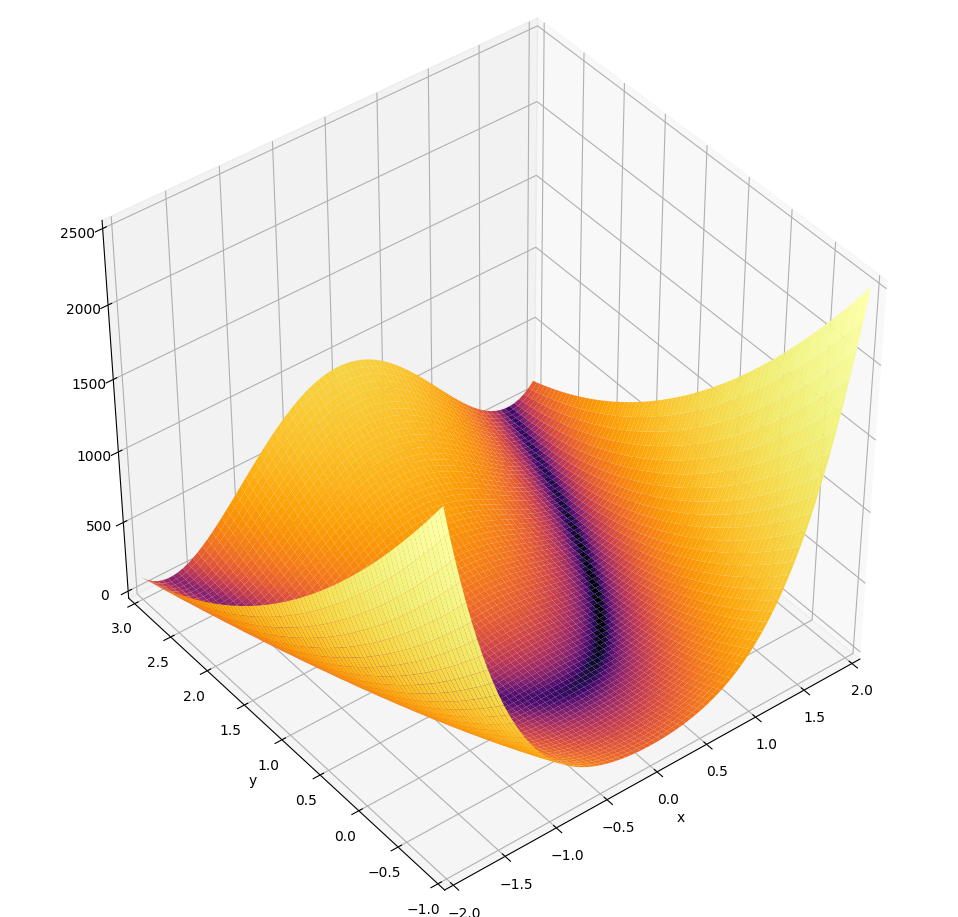
\includegraphics[height=5cm]{figures/Rosenbrock.png}
  \end{column}
\end{columns}
\end{frame}


\begin{frame}{Data Preprocessing Techniques}
\begin{columns}[c]
  \begin{column}{8cm}
  \begin{itemize}
    \item whitening transformation \\ $\rightarrow$ high range of rewards problematic
    \item normalization of samples and reward
  \end{itemize}
  \end{column}
  \begin{column}{6cm}
    \begin{figure}[h!]
      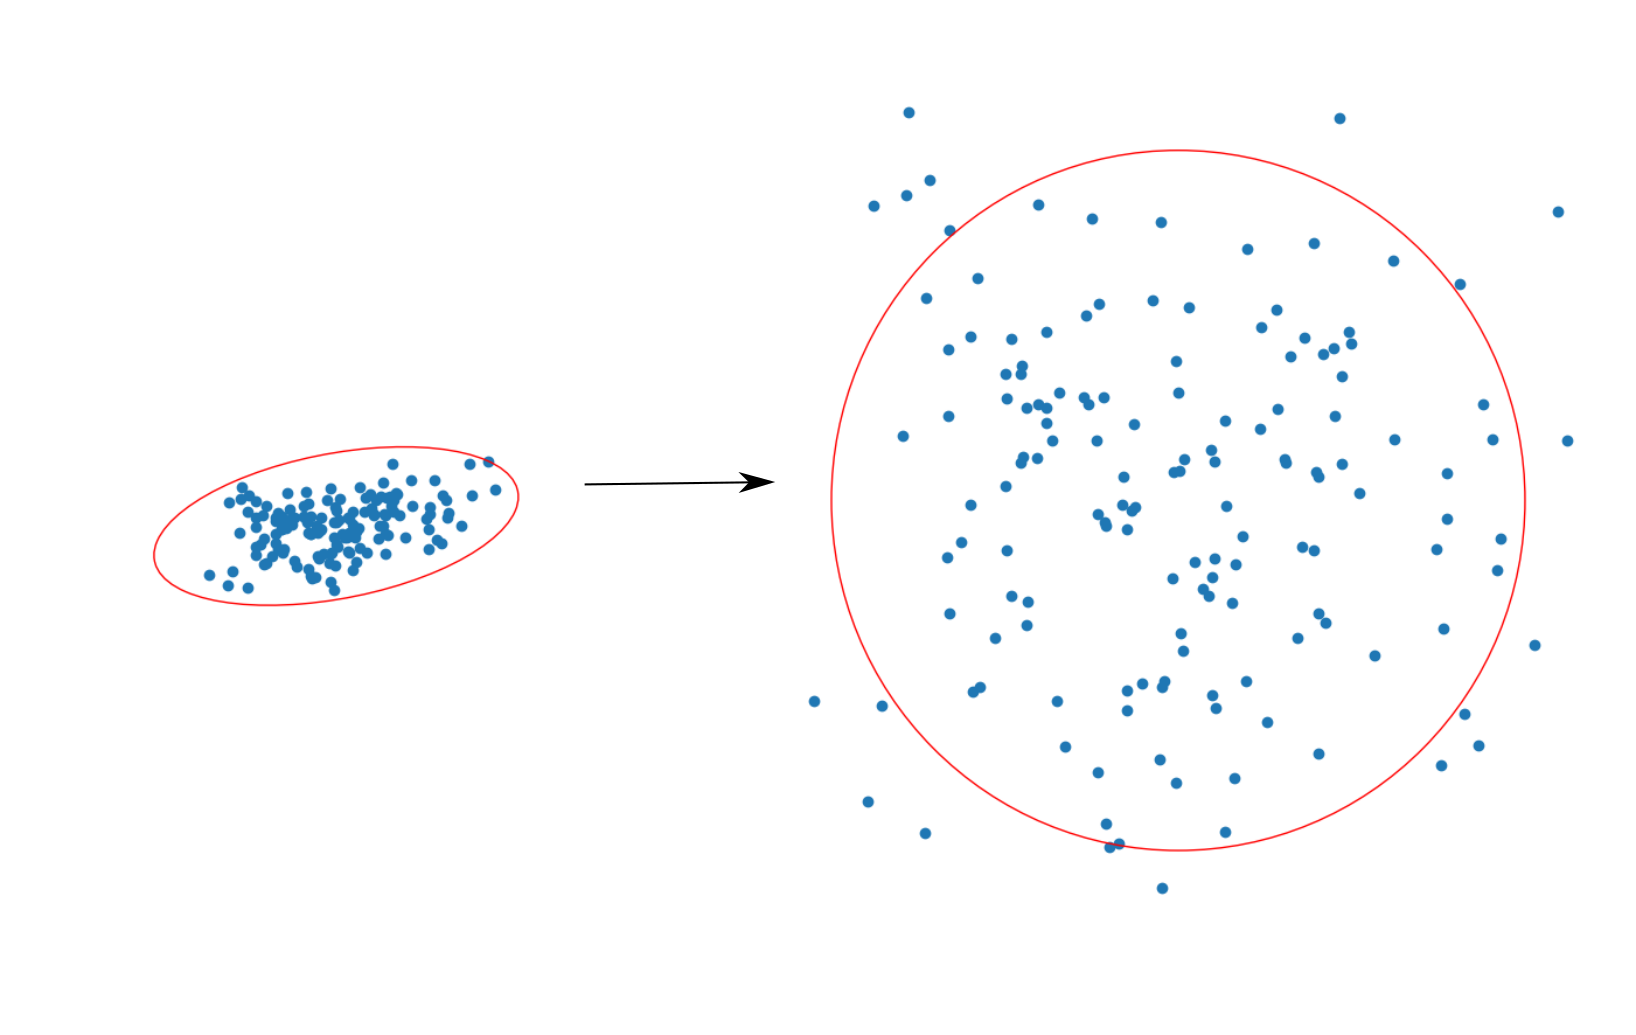
\includegraphics[height=4cm]{figures/white.png}
      \caption*{100 samples 2 dim Rosenbrock}
     \end{figure}
  \end{column}
\end{columns}  

\end{frame}


\begin{frame}{5 Dimensional Rosenbrock}
  \centering
  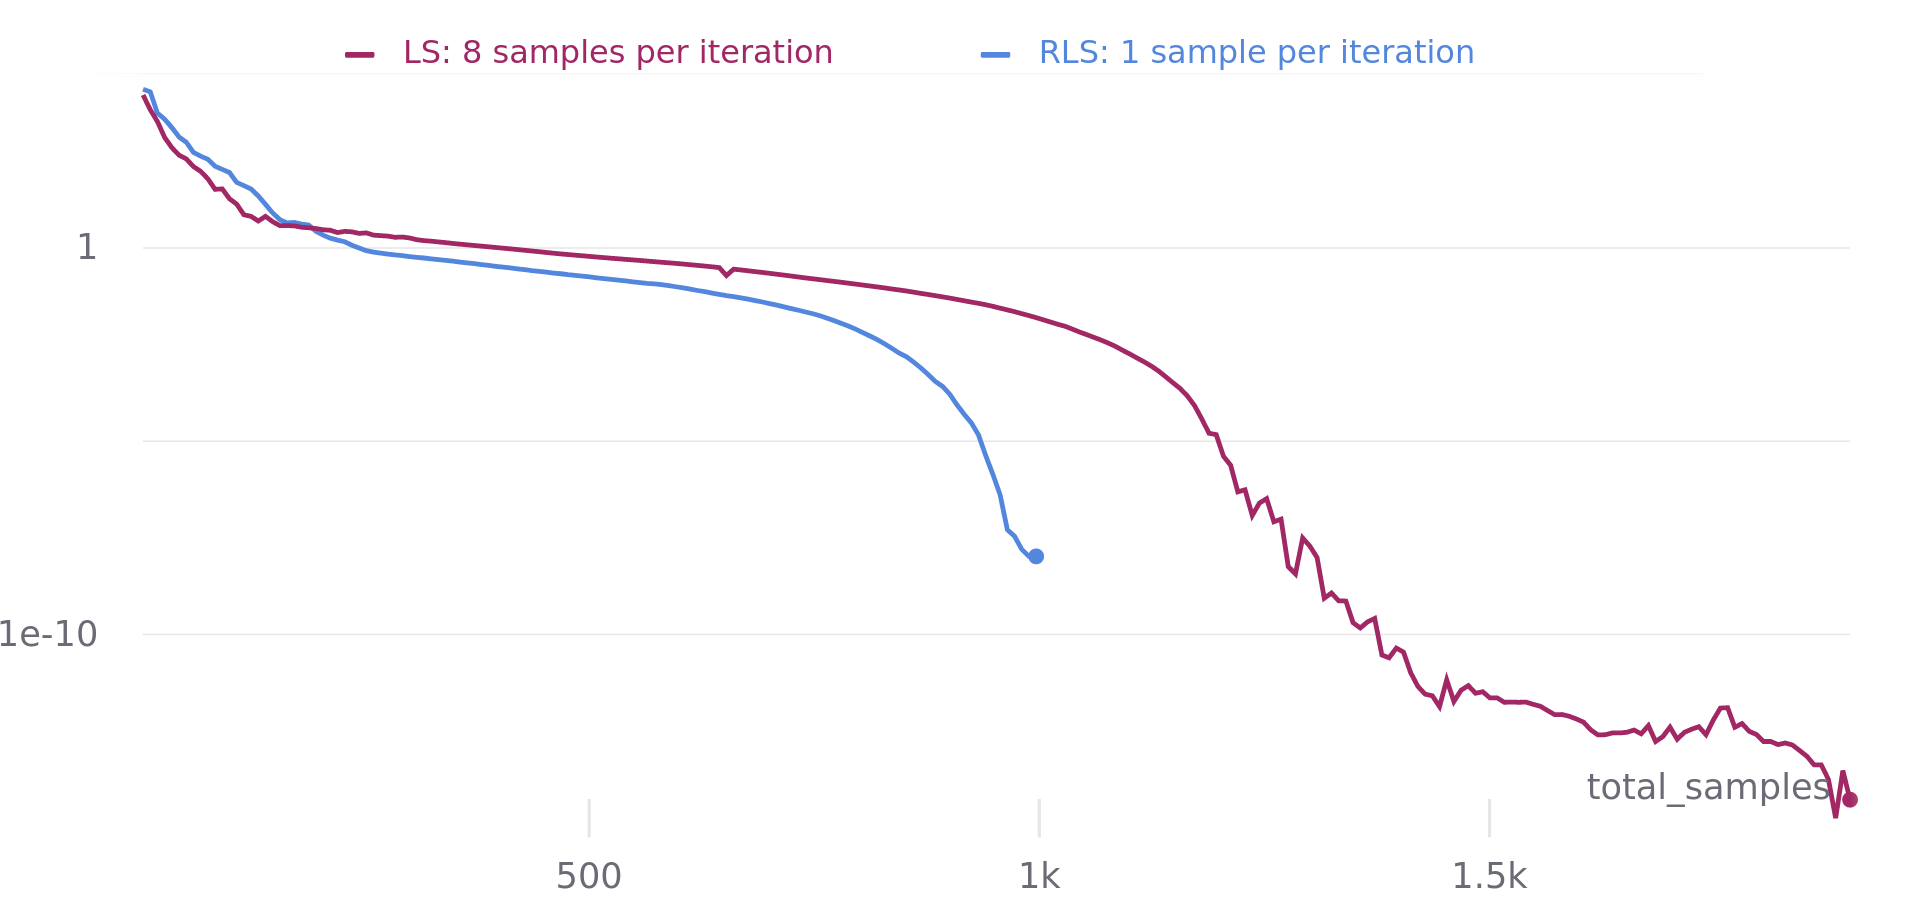
\includegraphics[height=6cm]{figures/totals_dim5.png}    
\end{frame}

\begin{frame}{5 Dimensional Rosenbrock}
  \centering
  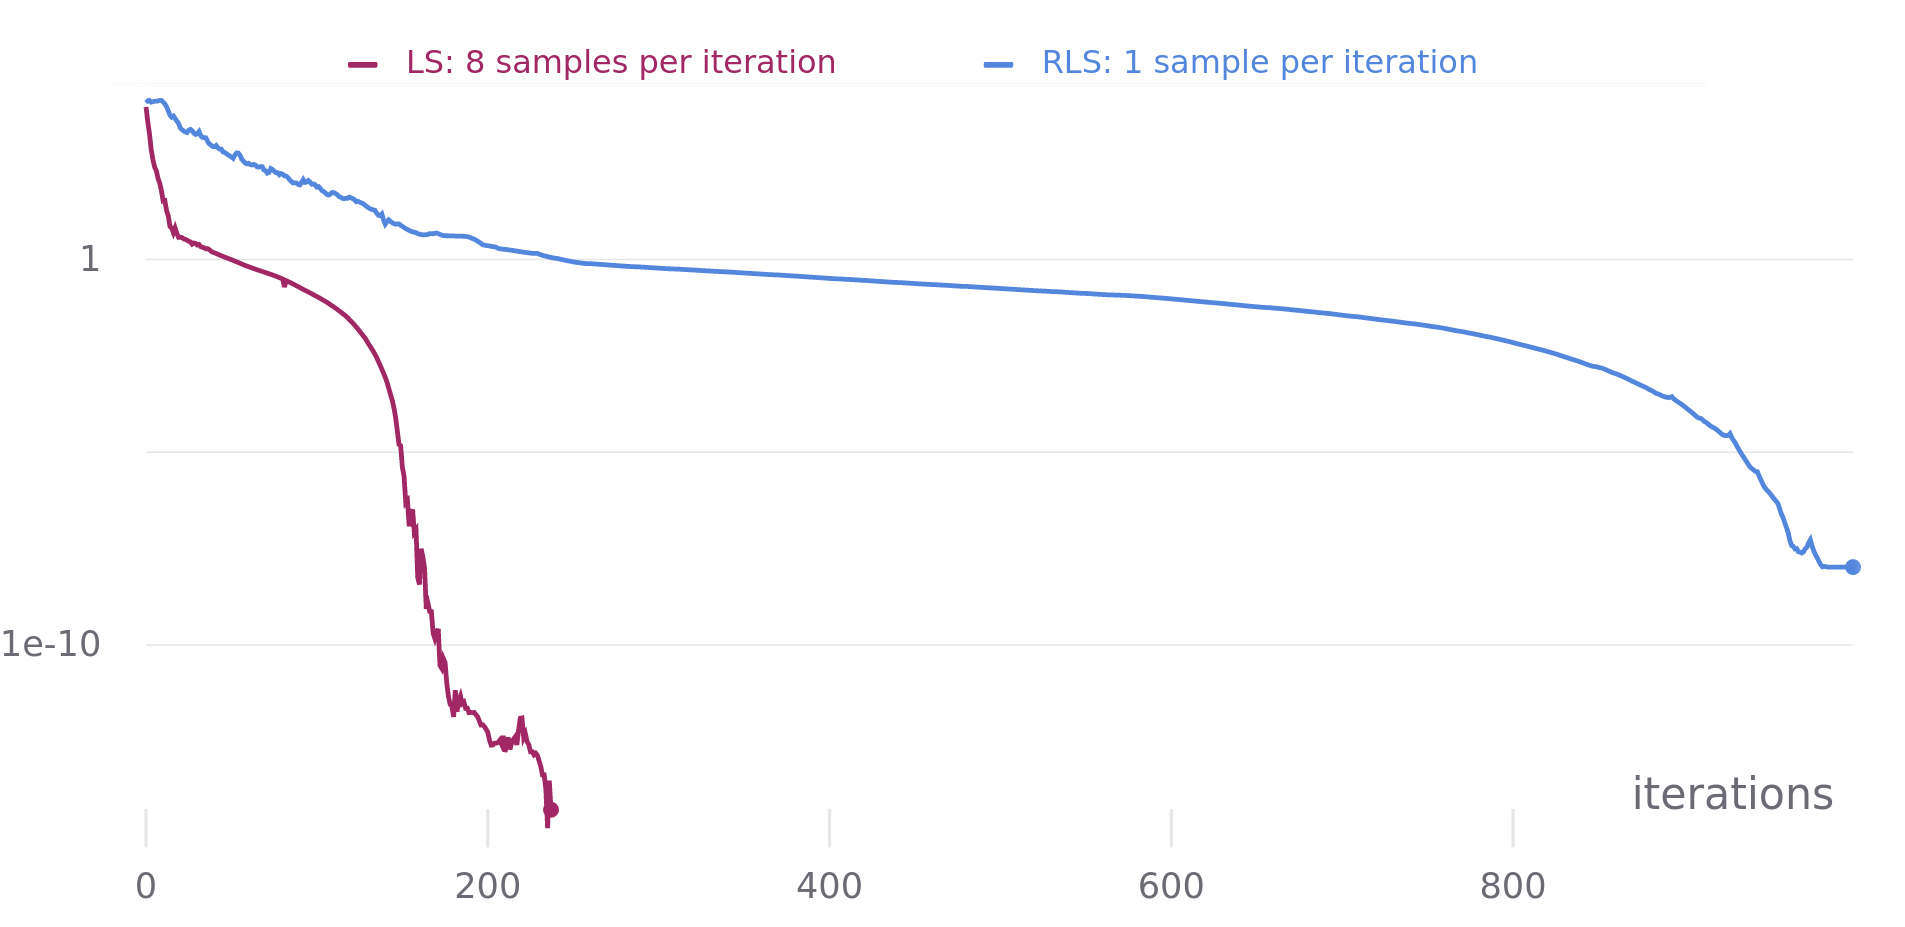
\includegraphics[height=6cm]{figures/iters_dim5.png}
\end{frame}


\begin{frame}{15 Dimensional Rosenbrock}
  \centering
  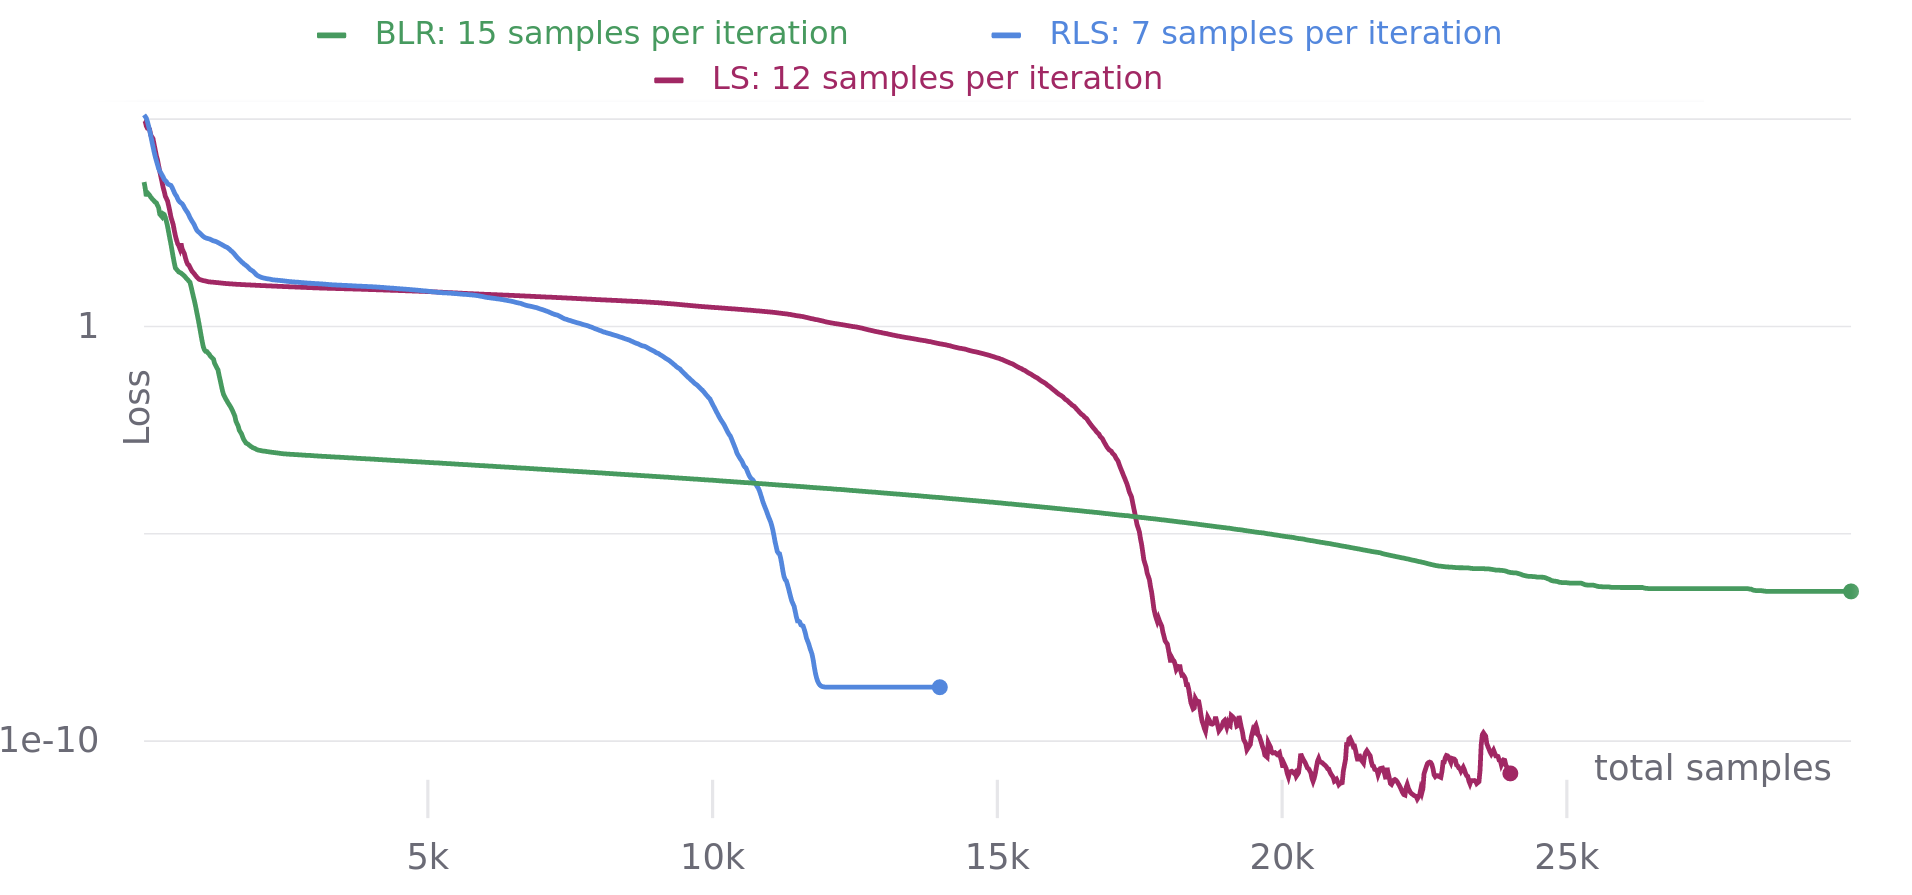
\includegraphics[height=6cm]{figures/total_all_15dim.png}
\end{frame}

%%%%%%%%%%%%%%%%%%%%%%%%%%%%%%%%%%%%%%%%%%%%%%%%%%%%%%%%%%%%%%%%%%%%%%%%%%%%%%%%
% only LS and RLS
% \begin{frame}{15 Dimensional Rosenbrock}
  % \centering
  % 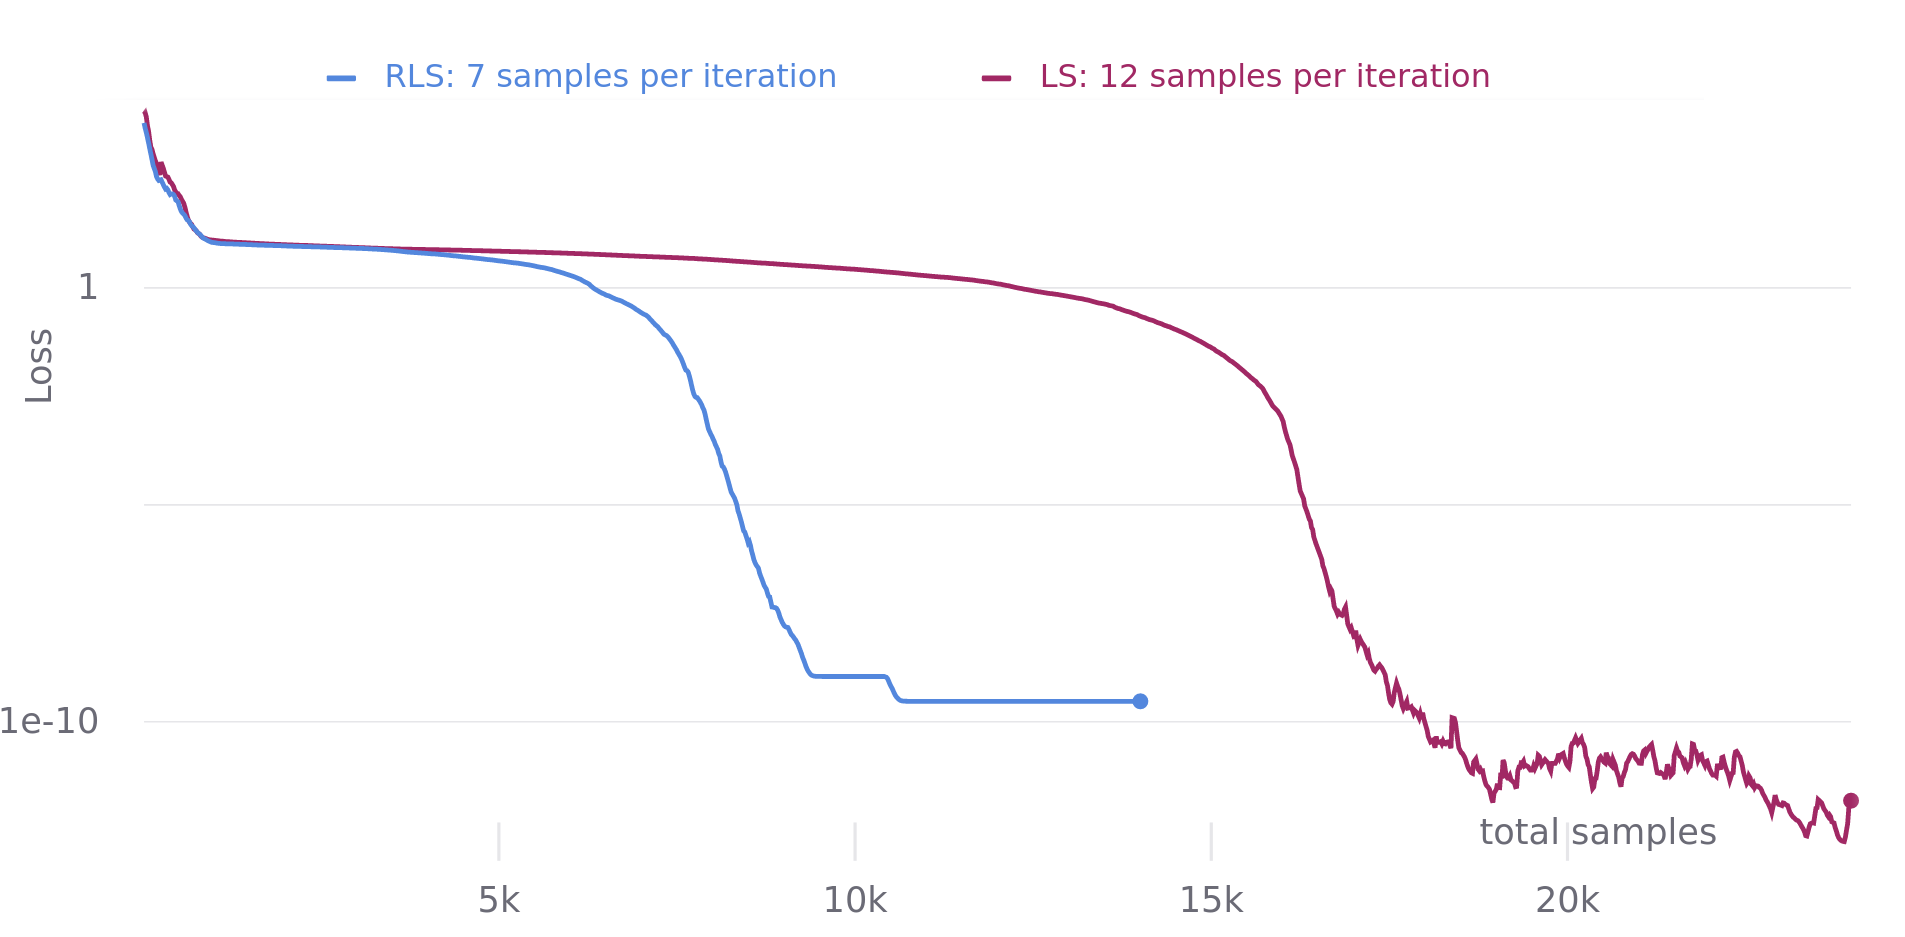
\includegraphics[height=6cm]{figures/total_dim15.png}  
% \end{frame}

% \begin{frame}{15 Dimensional Rosenbrock}
  % \centering
  % 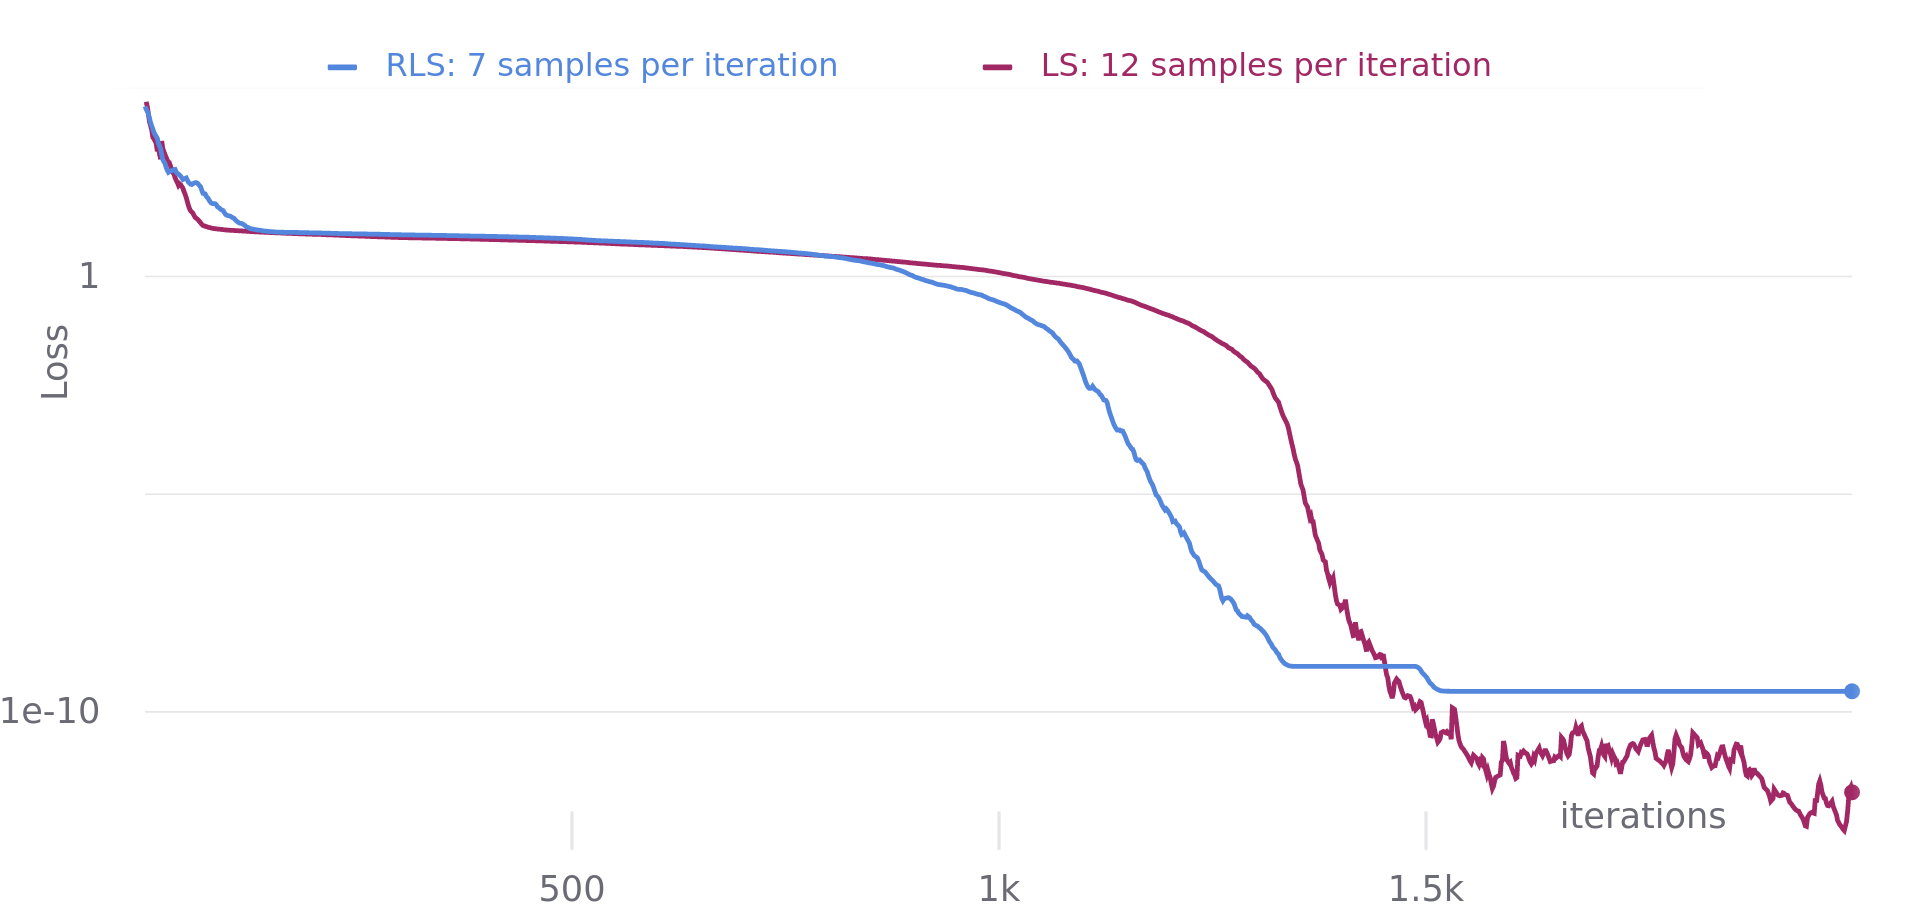
\includegraphics[height=6cm]{figures/iter_dim15.png}  
% \end{frame}
%%%%%%%%%%%%%%%%%%%%%%%%%%%%%%%%%%%%%%%%%%%%%%%%%%%%%%%%%%%%%%%%%%%%%%%%%%%%%%%%

%\begin{frame}{Results}
%TODO Rosenbrock dim 20 
%\end{frame}

%%%%%%%%%%%%%%%%%%%%%%%%%%%%%%%%%%%%%%%%%%%%%%%%%%%%%%%%%%%%%%%%%%%%%%%%%%%%%%%%
%%%%%%%%%%%%%%%%%%%%%%%%%%%%%%%%%%%%%%%%%%%%%%%%%%%%%%%%%%%%%%%%%%%%%%%%%%%%%%%%

\section{Outlook}
\begin{frame}{Outlook}

\begin{columns}[c]
  \begin{column}{9cm}
    \textbf{Problems:} \\
      \begin{itemize}
      \item constant parameter drift
      \item sample pool for RLS
      \end{itemize}
      $ $ \\
    \textbf{Next steps:} \\
    \begin{itemize}
      \item performance on other higher dimensional/noisy  objective functions?
      \item try to learn model parameter noise
      \item try planar reaching task
      \end{itemize}    
  \end{column}
  \begin{column}{5cm}
    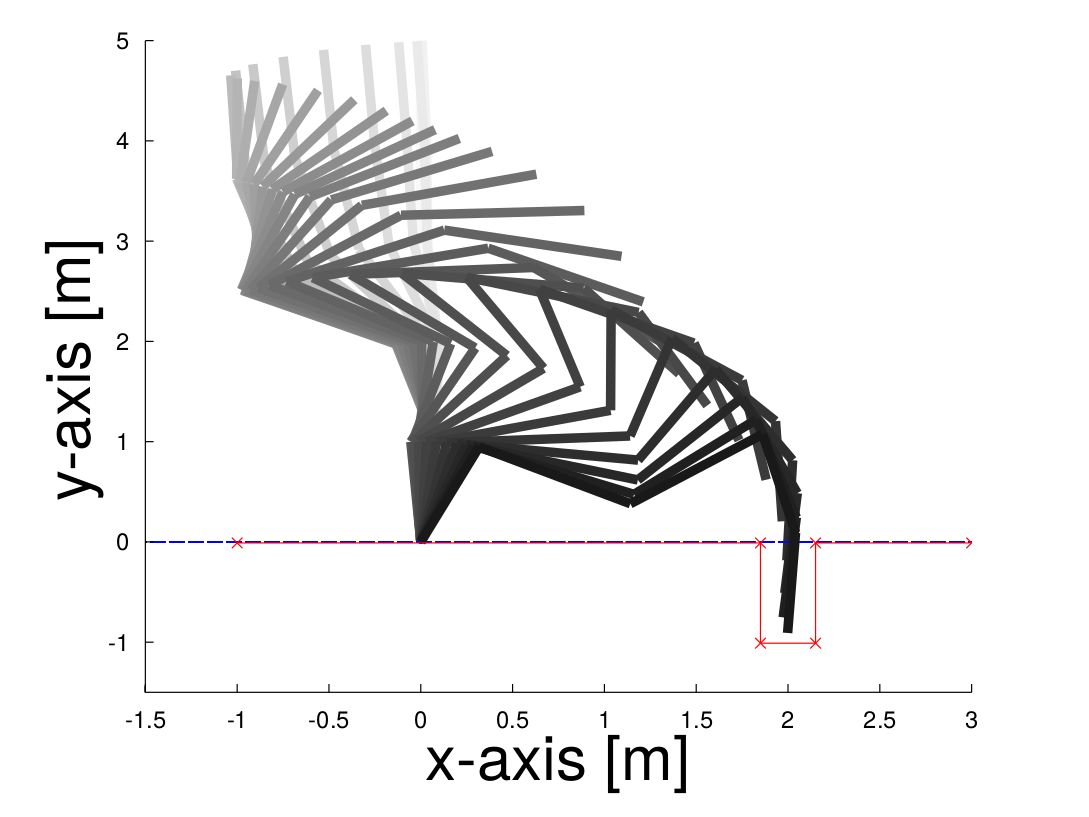
\includegraphics[height=4cm]{figures/hole_reaching.png}
  \end{column}
\end{columns}  

\end{frame}


% \begin{frame}{Conclusion}
  % \begin{itemize}
  % \item trying to improve \textcolor{blue}{sample efficiency} of MORE algorithm
  % \item first results show promise, but scale to higher dimension, complex tasks?
  % \end{itemize}
% \end{frame}

\begin{frame}{}
  \centering
  \huge
  Thank you! \\
  $ $ \\
  Discussion \& Questions?
\end{frame}

\appendix
\beginbackup

% \begin{frame}[allowframebreaks]{References}
% \printbibliography
% \end{frame}
\begin{frame}{15 Dimensional Rosenbrock}
  \centering
  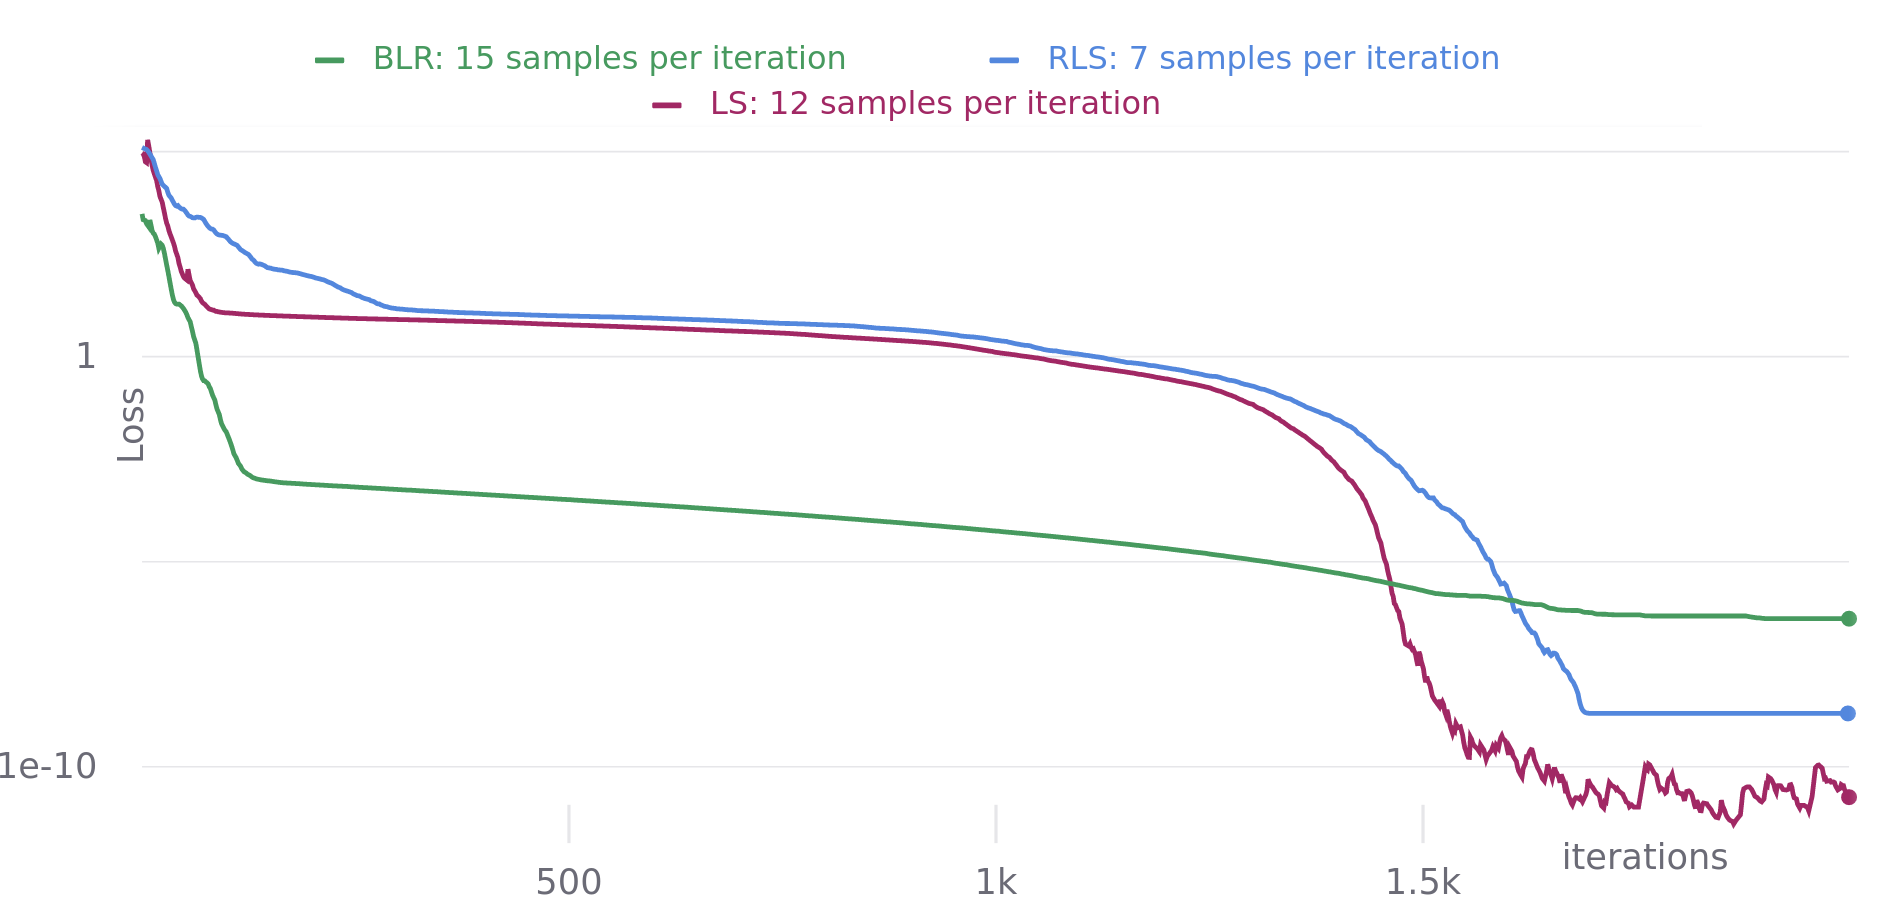
\includegraphics[height=6cm]{figures/iterations_all_dim15.png} \\
  Runtimes: LS $\sim$ 16 s, RLS $\sim$ 34s, BLR $\sim$ 11 min
  
\end{frame}


\begin{frame}{Drift model}
  Parameters perform Gaussian random walk:
  $$ p(\theta_k | \theta_{k-1}) = \text{N}(\theta_k | \theta_{k-1}, \textbf{Q}) $$ 
  Given:
$$ p(\theta_{k-1} | y_{1:k-1}) = N(\theta_{k-1} | m_{k-1}, P_{k-1})$$
  the joint distribution is (Markov assumption):
$$ p(\theta_k, \theta_{k-1} | y_{1:k-1}) = p(\theta_k | \theta_{k-1}) p(\theta_{k-1} | y_{1:k-1})$$

Use \textit{Chapman-Kolmogorov equation}:
$$ p(\theta_k | y_{1:k-1}) = \int p(\theta_k | \theta_{k-1}) p(\theta_{k-1} | y_{1:k-1}) d\theta_{k-1} $$
\end{frame}

\begin{frame}{MORE Algorithm details}
\begin{itemize}
\item Kullback Leibler Divergence
\end{itemize}
$$ D_{KL}(P||Q) = \int p(x) \text{ log} \frac{p(x)}{q(x)} dx $$
\end{frame}

\begin{frame}{MORE Theory}
$$ \mathcal{L}(\pi, \eta, \omega) = 
\int \pi(\theta) \mathcal{R}_{\theta} d\theta \; + \; 
\eta  \left(\epsilon - \int \pi(\theta) \text{ log}
 \frac{\pi(\theta)}{q(\theta)} d\theta\right)
 - \; \omega \left(\beta + \int \pi(\theta) \text{ log}(\pi(\theta)) d\theta\right)
$$

\textbf{Optimizing the Lagrangian}
$$ \pi^* = l(\eta,\omega) = \text{argmax}_{\pi} 
\mathcal{L}(\pi, \eta, \omega) $$

\end{frame}

\begin{frame}{Least Squares Equations}
    \begin{align*}
      p(\theta | y_{1:T}) &\propto p(\theta) \prod^T_{k=1} p(y_k|\theta)  \\
                          &= N(\theta | \textbf{m}_0, \textbf{P}_0)
                            \prod^T_{k=1} N(y_k | \textbf{H}_k \theta, \sigma^2)
    \end{align*}
    Because prior and likelihood are Gaussian, the \textit{posterior distribution} will
    also be Gaussian:
    $$ p(\theta | y_{1:T}) = N(\theta | \textbf{m}_T, \textbf{P}_T) $$
    
    \begin{align*}
      \textbf{m}_T &= [\textbf{P}_0^{-1} + \frac{1}{\sigma^2} \textbf{H}^T \textbf{H}]^{-1}
                     [\frac{1}{\sigma^2} \textbf{H}^T \textbf{y} + \textbf{P}_0^{-1} \textbf{m}_0] \\
      \textbf{P}_T &= [\textbf{P}_0^{-1} + \frac{1}{\sigma^2} \textbf{H}^T \textbf{H}]^{-1}
    \end{align*}

\end{frame}

\backupend

\end{document}